\chapter{提案手法} \label{chap:method}

%%%%%%%%%%%%%%%%%%%%%%%%%%%%%%%%%%
%    3Dモデリングにおけるエンティティ
%%%%%%%%%%%%%%%%%%%%%%%%%%%%%%%%%%
\section{データ構造}
サーバのデータを従来のテキストと同様に一次元に管理すると, 依存関係があった場合にデータの管理が困難となる.
3Dモデリングで用いるエンティティごとにデータを作成し, そのデータモデル間で依存関係を持つことによって解決する.
本システムでは3Dモデリングで用いるオブジェクト, 面, 頂点の3つのデータを定義し, 新しくデータを作成する場合, データベースにデータを登録していく仕様にした.
また, サーバデータとそのデータを各クライアントにコピーしたシャドウコピーを区別するために, シーンというデータを定義する.
図\ref{データ構造}にデータモデル間の依存関係を表した図を示す.
\begin{figure}[htbp]
  \begin{center}
    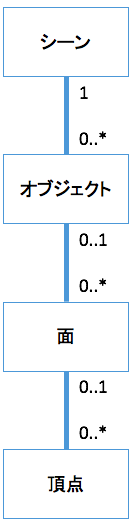
\includegraphics[scale=0.5]{images/er}
    \caption{データモデル間の依存関係}
    \label{データ構造}
  \end{center}
\end{figure}
% TODO 足りない
図\ref{データ構造}のようにシーンのデータはオブジェクトを, オブジェクトは面を, 面は頂点をそれぞれ子にもつ. また, 子のみが親の参照先をもつ.

このデータ構造によって, 子を削除した場合に親との依存関係も削除できる.親を新しく設定する場合, 子のデータを複製しながらそれぞれに新しく設定する親を参照先に設定する.
子のデータを複製していくことによって, 関係を削除した際も複製元のデータは残る.

%%%%%%%%%%%%%%%%%%%%%%%%%%%%%%%%%%
%    同期の手順
%%%%%%%%%%%%%%%%%%%%%%%%%%%%%%%%%%
\section{同期の手順}
同期はDifferential Synchronizationに基づいて行う.
同期の手順を具体的な例を用いて説明する. クライアントAは新しく頂点``101xyz''
を作成し, その後, クライアントBは既にある頂点``100abc''を削除する.
クライアントAの同期の手順を図\ref{sycle1}に示す.
クライアントAが編集を行うと, クライアントAのクライアントデータに``101xyz''が作成される図\ref{sycle1}(a).
また, 一定時間ごとに同期の処理を行う. クライアントAでは, 差分を計算し, [+ ``101xyz'']となる. [+ ``101xyz'']をクライアントAのサーバシャドウと, サーバデータに適用する図\ref{sycle1}(b). その時クライアントAではクライアントデータをクライアントシャドウにシャドウコピーする図\ref{sycle1}(c). サーバでは差分を計算し, 差分なし[ ]となる図\ref{sycle1}(d). この際にサーバではサーバデータをクライアントAのサーバシャドウにシャドウコピーする図\ref{sycle1}(e).
\par
クライアントBの同期の手順を図\ref{sycle2}に示す.
クライアントBが編集を行うと, クライアントBのクライアントデータにある``100abc''を削除する図\ref{sycle2}(a).
また, クライアントAと同様に一定時間ごとに同期の処理を行う. 差分を計算し, [-- ``100abc'']となる. [- ``100abc'']をクライアントBのサーバシャドウと, サーバデータに適用する図\ref{sycle2}(b). その時クライアントBではシャドウコピーする図\ref{sycle2}(c). サーバでは差分を計算し, [+ ``101xyz'']となる. [+ ``101xyz'']をクライアントBのクライアントデータとクライアントシャドウに適用する図\ref{sycle2}(d). この際にサーバではシャドウコピーする図\ref{sycle2}(e).
本来, 変数v1を変数v2にシャドウコピーするならばv2 = v1のように代入することで実装する. しかし, 本システムではデータをデータベースに登録して管理しており, 単純な代入で処理できない.
また, 元のデータを削除し新しくシャドウコピーを作成する方法は, 頻繁にシャドウコピーを行うDifferential Synchronizationでは,
データベースのDELETE命令とCREATE命令を頻発させることになり, 処理においてボトルネックとなってしまう. サーバでのシャドウコピーは, サーバデータとサーバシャドウの差分を取り, サーバシャドウに適用することによって解決する.
\begin{figure}[htbp]
  \begin{center}
    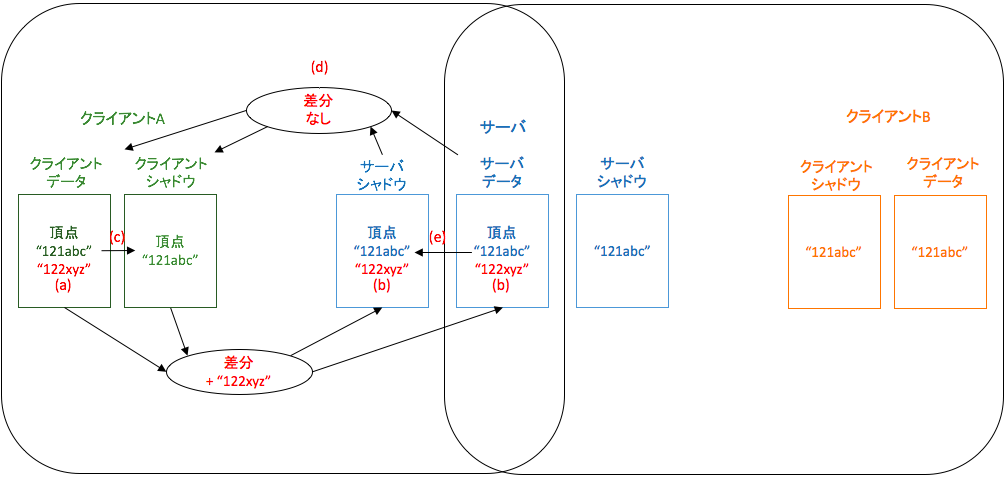
\includegraphics[scale=0.3]{images/sycle1}
    \caption{クライアントAの同期の手順}
    \label{sycle1}
  \end{center}
\end{figure}
\begin{figure}[htbp]
  \begin{center}
    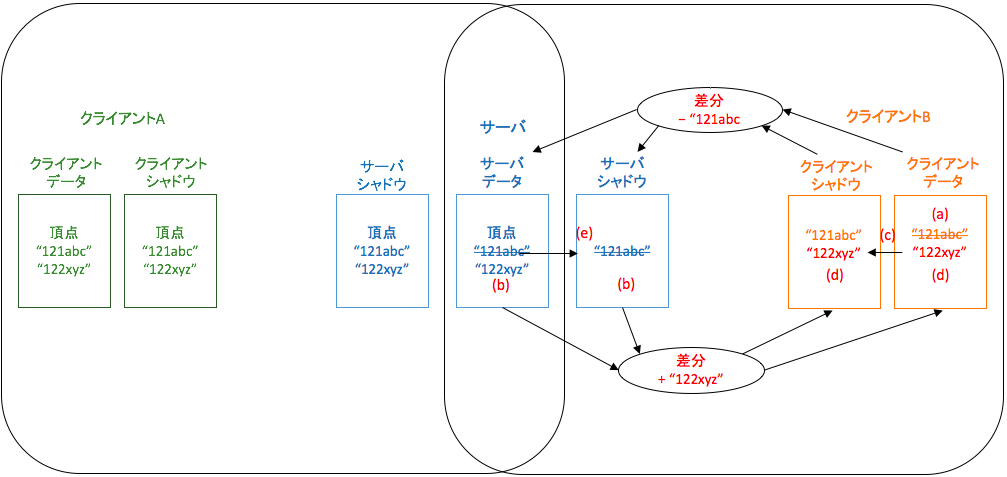
\includegraphics[scale=0.3]{images/sycle2}
    \caption{クライアントBの同期の手順}
    \label{sycle2}
  \end{center}
\end{figure}
%%%%%%%%%%%%%%%%%%%%%%%%%%%%%%%%%%
%    固有IDの付与
%%%%%%%%%%%%%%%%%%%%%%%%%%%%%%%%%%
\section{固有IDの付与} \label{固有id}
各データには, 複数クライアント間でIDの衝突が起こるのを防ぐため, そのデータを作成したクライアント識別子を組み込んだ固有IDを与える.
本システムでは図\ref{uuid}のように, クライアント識別子--データモデル識別子--インクリメント番号--ランダム文字列の順につなげた固有IDを与える. クライアント識別子は1から順に振られたユーザIDを用いてクライアントが付与する. また, データモデル識別子は, オブジェクトが0, 面は1, 頂点は2となるように与える. サーバでもクライアントでも作ったデータの数を記憶しておき, 作るごとにインクリメントするインクリメント番号を固有IDに組み込む.
\begin{figure}[htbp]
  \begin{center}
    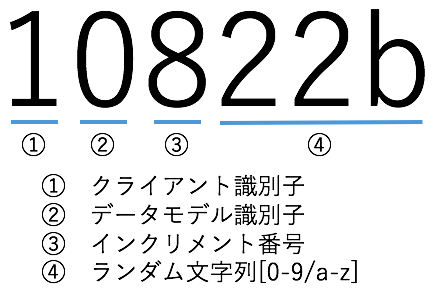
\includegraphics[scale=0.5]{images/uuid}
    \caption{本システムの固有ID}
    \label{uuid}
  \end{center}
\end{figure}
%%%%%%%%%%%%%%%%%%%%%%%%%%%%%%%%%%
%    基本命令
%%%%%%%%%%%%%%%%%%%%%%%%%%%%%%%%%%
\section{基本命令} \label{ope}
オブジェクト, 面, 頂点の各データモデルに対して, 作成, 親への参照の追加, 削除の3つの基本命令を定義する.
これらの命令はシステムに対する最低限の基本命令であり, これらの命令を組み合わせることで, 3Dモデリングで使われる面の分割や押し出しなど, より高度な命令を実現できる.
削除命令や親への参照の追加をする命令を適用する際, 操作対象が他の命令で削除されていた場合は命令を無効とする.
